\chapter[Materiais e métodos]{Materiais e métodos} \label{chap:materials-and-methods}

Tendo entendido os conceitos básicos para o entendimento da abordagem do trabalho e toda sua problemática, deve-se então entender melhor como será desenvolvido o trabalho e como a metodologia foi estruturada. Portanto, o presente capítulo visa mostrar os materiais e metodologia visando clarear e demonstrar, desde a identificação do dado a ser utilizado, como será o processo para a geração de modelos de IA, bem como os insumos utilizados e as métricas de validação identificadas.

\section{O dado} \label{sec:dataset}

Como dito, existem diversos tipos de áreas de desenvolvimento inseridos no termo Inteligência Artificial. A área de \textit{machine learning} é caracterizada pela capacidade da máquina aprender a partir de experiências com o dado, por isso deve-se dar uma enorme importância para a qualidade do dado para conseguir resolver problemas com ML, mais ainda para \textit{Deep Learning}. Para ser possível a construção de um modelo que visa testar a hipótese de estudo em questão, seria necessário realizar o levantamento de um conjunto de dados em formato de texto, em português, que fosse possível alimentar o modelo a ser criado.

O Grupo de Pesquisa em Aprendizado de Máquina (GPAM) da Universidade de Brasília desenvolveu em 2018 um projeto de pesquisa que visa realizar a classificação das repercussões gerais do Supremo Tribunal Federal (STF) \cite{cnn-for-STF}. Para essa classificação, o projeto precisava realizar a extração de informações dos textos das decisões judiciais do STF, sendo essas possuindo documentos digitais tanto formulados digitalmente, manuscritos e/ou escaneados. Tal conjunto de dados foi fornecido para o presente trabalho de conclusão a fim de facilitar o processo de aquisição dos mesmos por meio de \textit{crawlers}\footnote{
  \textit{Crawlers} ou \textit{web crawlers} são tecnologias que possibilitam a extração de informações disponíveis em sites da Internet de maneira organizada para possibilitar o consumo desses dados para desenvolvimento de algoritmos. Bastante comum para criação de base de dados de ML.
} ou outras fontes.

\subsection{Características}

Foram fornecidos 89.578 processos do Supremo Tribunal Federal em formato PDF, contendo os diversos temas de repercussões gerais e diferentes características \cite{cnn-for-STF}. Algumas delas são:

\begin{itemize}
  \item O STF recebe processos em segunda instância de todo o Brasil e não existe nenhum padrão em sua formatação, fonte, espaçamento e escrita;
  \item Uma parte significante dos documentos fornecidos estão em forma de imagem obtidas por meio de \textit{scanners} e muitas vezes possui anotações, estampas, marcas d'agua, manchas, sombras, etc.
\end{itemize}


No projeto desenvolvido, o GPAM realizou um conjunto de extrações e formatações dos documentos para facilitar o trabalho a partir de uma etapa de processamento.

\begin{figure}[H]
  \centering
  \caption{Fluxo de processamento de processos do STF pelo GPAM.}
  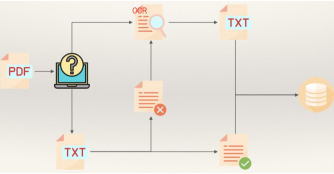
\includegraphics[width=13cm, center]{figuras/gpan-pipeline.png}
  \legend{Fonte: \citeonline{cnn-for-STF}}
  \label{fig:gpan-pipeline}
\end{figure}

Nesse processamento, uma das etapas consistiu em verificar se a página do documento possui texto selecionável ou não, para então realizar a extração do texto via algoritmo de OCR. Tudo isso foi armazenado em um arquivo CSV, cuja as principais estão descritas a seguir.

% process_id,,,,,document_id,,,page_is_ocr,,page_text_extract,page_number,,

\begin{table}[h]
 \centering
 \caption{Principais características do dado CSV}
 \begin{tabular}{|m{9em}|m{20em}|}
    \hline
      \textbf{Coluna}  &
      \textbf{Descrição} \\
    \hline
      \textit{process\_id}  &
      Parte do número do processo no tribunal \\
    \hline
      \textit{document\_id}  &
      Identificador do documento dentro do processo \\
    \hline
      \textit{page\_is\_ocr}  &
      Booleano definindo se a página necessita de OCR \\
    \hline
      \textit{page\_text\_extract} &
      Texto extraído da página utilizando OCR \\
    \hline
      \textit{page\_number} &
      Número da página do PDF a qual aquela extração pertence \\
    \hline
 \end{tabular}
 \legend{Fonte: autoral}
 \label{tab:csv-details}
\end{table}

É importante notar que os campos \textit{process\_id} e \textit{document\_id} se repetem no CSV mas a junção de ambos juntamente com a \textit{page\_number} identificam unicamente a página dentro do PDF.

\section{A métrica}

A métrica a ser utilizada deve ser capaz de realizar a comparção do OCR da imagem original entre a imagem com ruído com o OCR da imagem original entre a imagem gerada. Para provar a hipótese em questão, se for validada, a métrica de comparação deve dizer que o OCR da imagem gerada está mais próximo do que o da imagem com ruídos, provando assim a geração de uma imagem melhor do que a imagem ruim. Com isso em mente, deve-se considerar métricas de análise e comparação de texto puro, ignorando as métricas de performance de OCR que visam analizar a qualidade do algoritmo de segmentação e extração de texto de imagem.

Nos sistemas de sumarização de texto, processo pelo qual gera-se um texto a partir de outro utilizando \textit{Machine Learning}, tradicionalmente envolve julgamentos humanos de diferentes métricas de qualidade para a identificação de coesão, coerência, concisão, gramática, etc \cite{automatic-summarization}, o que acaba sendo muito custoso para realizar isso manualmente. Com isso, \citeonline{rouge-metric} propôs uma nova métrica que tentasse realizar esse tipo de avaliação de maneira automatizada, chamada \textit{Recall-Oriented Understudy for Gisting Evaluation} (ROUGE). Esse método de avaliação possui quatro (4) diferentes maneiras de se avaliar a diferença de um texto original ao gerado pela sumarização. Porém, alguns desses são utilizados quando se tem dois textos de sumarização gerados sendo comparados com o texto original ou que permite uma "falha" entre uma sumarização sem perder a informação geral, o que foge um pouco do escopo e da ideia apresentada. Os que serão utilizados são mostrados a seguir.

\subsection{ROUGE-N: N-Grama de Co-Ocorrência}
Essa métrica é capaz de identificar a ocorrência de n-gramas repetidos entre um texto candidato (gerado) e um texto referência. Um n-grama é um conjunto de palavras, onde 1-grama agrupa uma única palavra (unigrama), 2-grama define um grupo de duas palávras (bigrama), etc. Tal métrica é calculada da seguinte maneira:

\begin{gather}
  ROUGE{-N} = \frac{\sum_{r} . \sum_{n} match(gram_{n})}
  {\sum_{r} . \sum_{n} count(gram_{n})}
\end{gather}

Onde $n$ é o tamanho do n-grama $gram_n$, $match(gram_{s,})$ é o número máximo de n-gramas que ocorrem tanto no texto gerado quanto no texto de referência e $r$ é o número de textos candidatos. Quando maior o número de n-gramas identificados no texto candidato, maior é o valor da métrica ROUGE-N. A métrica pode ser expandida para a comparação entre um candidato e multiplas referências. Como no caso existe apenas uma referência, essa evolução não será apresentada.

Essa é a métrica mais indicada para a comparação de sobreposição de n-gramas.

\subsection{ROUGE-L: Maior Subsequência Comum}

Essa métrica, do inglês \textit{Longest Common Subsequence} ou LCS diz que, dada duas sequências $X$ e $Y$, a maior subsequência comum (LCS) de $X$ e $Y$ é uma subsequência\footnote{
  A sequência \(Z = [z_1, z_2, ..., z_n]\) é uma
  subsequência de \(X = [x_1, x_2, ..., x_m]\) se existir uma estrita sequência crescente \([i_1, i_2, ..., i_k]\) de indices de $X$ onde para todo \(j = 1, 2, ..., k\), se tem \(x_{i,j} =  z_j\) \cite{intro-to-algorithms}.
} com o tamanho máximo.

Para a verificação da LCS em um texto de sumarização, considera-se uma sentença do sumário como uma sequência de palvras. Com isso, a intuição é que quanto maior o LCS de duas sentenças são, maior será a similaridade dos dois textos. Propõe-se então o uso de uma LCS baseada em mensuração F para estimar a similaridade entre dois textos $X$ de tamanho $m$ e $Y$ de tamanho $n$, assumindo que $X$ é o texto original de referência e $Y$ é o texto gerado.

\begin{gather}
  R_{lcs} = \frac{LCS(X, Y)}{m}
\end{gather}

\begin{gather}
  P_{lcs} = \frac{LCS(X, Y)}{n}
\end{gather}

\begin{gather}
  F_{lcs} = \frac{(1 + \beta^2).R_{lcs} . P_{lcs}}{R_{lcs} + \beta^2.P_{lcs} }
\end{gather}

Onde \(LCS(X, Y)\) é o tamanho da maior subsequência comum entre $X$ e $Y$, \(\beta = \frac{P_{lcs}}{R_{lcs}}\) quando \(\frac{\partial F_{lcs}}{\partial R_{lcs}} = \frac{\partial F_{lcs}}{\partial P_{lcs}}\). Se \(X = Y\), então a ROUGE-L é 1, mostrando que os textos são praticamente os mesmos. Quanto mais próximo de 0, mais distantes os textos são.

\ornament

Por se tratarem de métricas de análise de texto, tendo como base o texto original, pode-se fazer uma analogia ao problema tratado no presente trabalho, onde realiza-se a comparação entre o texto extraído de um OCR tanto de uma imagem boa (original) quanto de imagens ruins e imagens geradas. Portanto, essa será a métrica de avaliação utilzada na etapa de validação da hipótese.

\section{Método proposto}

Para a criação de qualquer projeto científico deve-se seguir ou criar um método de trabalho que possibilite a construção de uma solução que consiga mostrar, de maneira clara e objetiva, o trabalho realizado para a comprovação, validação ou invalidação da hipótese apresentada.

Portanto, no presente projeto desenvolveu-se uma metodologia que possibilite validar se um modelo gerador de ML consegue melhorar a qualidade do OCR de fotos ruins. Tal método é dividido diferentes frentes que vão desde trabalho e curadoria do dado até a análise de métricas de qualidade de OCR, permitindo assim a comparação dos diferentes resultados encontrados pelos modelos de IA criados, bem como compará-los com o processamento de imagem simples para possíveis correções em etapas de pré-processamento pelas ferramentas de OCR.

\subsection{Geração de \textit{dataset}}

Essa etapa consiste em relizar uma análise sobre os dados fornecidos pelo GPAM para que seja possível, considerando a diferente problemática pelo qual o dado já foi utilizado, construir uma base de dados sólida e que seja adequada ao problema em questão. Tal etapa será dividida em 4 (quatro) vertentes, sendo essas mais detalhadas em sequência, melhor identificados na figura \ref{fig:crappy-flow-diagram}.

\begin{figure}[H]
  \centering
  \caption{Processo para a criação de \textit{dataset}.}
  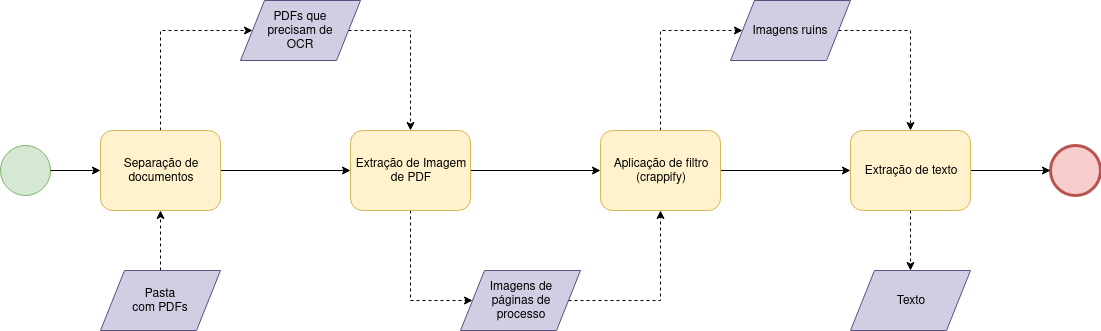
\includegraphics[width=\linewidth, rotate=0]{figuras/crappy-flow-diagram.png}
  \legend{Fonte: autoral}
  \label{fig:crappy-flow-diagram}
\end{figure}

O principal objetivo da presente fase da metodologia é conseguir criar imagens \textit{crappy}, ou seja, fotos que sofreram um processamento de imagem para piorar sua qualidade com diferentes tipos de aplicação de filtros e que consequentemente dificultam - não impossibilitando - o trabalho do algoritmo de reconhecimento de caracteres.


\subsubsection{Separação de documentos} \label{sssec:documents-split}

Nessa etapa, recebe-se como entrada a pasta com todos os PDFs fornecidos pelo GPAM e o principal objetivo dela é conseguir extrair e identificar algumas características sobre o dado a ser trabalhado.

Aqui, será possível identificar, dentro da amostra de dados, quais serão os PDFs que possuem páginas que necessitam de extração via OCR para assim separar os mesmos entre "necessitam de OCR" \  e "não necessitam de OCR". Aqueles processos que não necessitarem de OCR para a extração de conteúdo serão inicialmente ignorados no presente trabalho, sendo utilizados apenas na possível identificação de necessidade de mais dados para treinamento.


\subsubsection{Extração de imagem do PDF}

Obtendo os PDFs que necessitam de OCR a partir do processamento na etapa \ref{sssec:documents-split}, será possível realizar a extração das páginas específicas dentro do PDF que necessitam da extração com o reconhecimento de caracteres. Com isso, propõe-se o uso da tecnologia \textit{pdf2image}, biblioteca implementada em Python que possibilita tal atividade.

Essa ferramenta possibilita criar uma imagem a partir de uma página de PDF, funcionando como um \textit{scanner}, mantendo a qualidade da página do PDF, incluindo suas cores e tamanho.

A saída dessa etapa consistirá em todas as fotos necessárias para a criação de imagens \textit{crappy}, descritas na sequência.


\subsubsection{Aplicação de filtros}

Obtendo todas as imagens de páginas que precisam de OCR para a extração de conteúdo, será então iniciada a etapa de "\textit{crappify}" \  de imagens, ou seja, transformar imagens de boa qualidade em imagens ruins.

Para a realização dessa transformação e geração de imagens \textit{crappy}, serão estudados métodos que possibilitem, a partir de processamento de imagem, aplicar ruídos, reduzir qualidade, sombreados, etc, para que seja possível simular imagens escaneadas de pior qualidade que são vistas diariamente pelos trabalhadores da área jurídica.

Tendo identificado e levantado as bibliotecas que possibilitem a geração de imagens ruins, bem como a criação de algoritmos autorais para tal, será proposta uma \textit{pipeline} "\textit{crappier}" \  de imagens, para que seja possível a criação das imagens \textit{crappy}.


\subsubsection{Extração via OCR de imagens \textit{crappy}}

Para que seja possível criar uma métrica que sirva para a verificação da qualidade do OCR, deve-se ter tando extrações de textos de imagens boas e ruins que possibilite comparar ambas as extrações. Com isso, a partir das imagens a serem criadas na etapa anterior, será possível realizar a extração de texto das imagens ruins.

Nessa etapa, idealiza-se extrair o texto de todas as imagens \textit{crappy} e armazena-las de maneira organizada para que essas possam ser utilizadas futuramente nas métricas.

Para tal extração, a ferramenta que será utilizada é o Tesseract com configuração em português, já disponibilizada pela comunidade.


\subsection{Gerador de Imagens}

Essa etapa consiste em desenvolver um modelo de IA que receba como entrada uma imagem ruim e gere uma nova imagem nunca vista antes. Essa imagem será gerada a partir de uma Rede Neural Convolucional, como já foi citado na seção \ref{ssec:generative-vs-discriminative}.

\begin{figure}[H]
  \centering
  \caption{Simulação de geração de imagem a partir de modelo Gerador}
  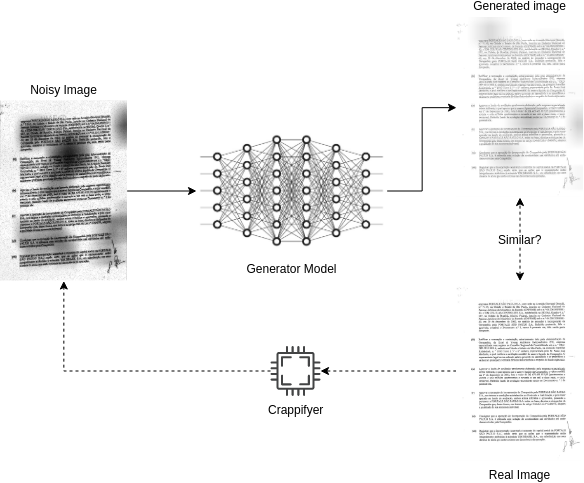
\includegraphics[scale=0.6]{figuras/image-generation.png}
  \legend{Fonte: autoral}
  \label{fig:image-generation}
\end{figure}

Idealiza-se então realizar os testes com os modelos citados na sessão \ref{ssec:generative-vs-discriminative}. Por se tratar de abordagens diferentes de modelos geradores utilizando \textit{Deep Learning}, será realizado uma comparação dos diferentes resultados que provavelmente serão encontrados a partir dos modelos geradores.


% Tendo uma nova imagem gerada e todas as informações necessárias identificadas previamente, como OCR das imagens boas e ruins, adiciona-se uma camada de extração de texto das imagens geradas pelo modelo Gerador e as adiciona no CSV contendo as extrações anteriores. Com isso, tem-se agora o insumo necessário para a criação de uma métrica de validação da hipótese.


% \section{Cronograma de desenvolvimento}

% Para a simplificação do entendimento da metodologia proposta, bem como para melhorar a organização e divisão do trabalho, foi desenvolvido um cronograma simples que visa mostrar de forma tabelar as atividades a serem desenvolvidas. Tais atividades foram divididas em dois momentos, correspondendo às duas entregas necessárias para a finalização do trabalho.

% Identificar todas as micro-atividades desenvolvidas e descrever todas elas seria massivo e dificultaria o entendimento. Por isso, ao invés de propor datas e detalhar cada uma das micro-atividades, o cronograma é baseado em macro-atividades, divididas em \textit{sprints} simplificadas, ou seja, sem atividades de revisão e planejamento documentadas. Uma \textit{sprint} é uma atividade proposta pela metodologia Scrum que possibilita o desenvolvimento interativo e incremental por meio de atividades com definição de tempo e entregas específicas \cite{scrum}.

% \subsection{Momento 1}

% O momento 1 representa todas as atividades que fazem parte do escopo da entrega 1, referente às etapas que vão desde o recebimento dos dados até a criação do \textit{dataset} que servirá de insumo para as fases do momento 2. As atividades e suas respectivas \textit{sprints} estão identificadas na tabela \ref{tab:step-1}

% \begin{table}[H]
%   \centering
%   \caption{Cronograma de atividades do momento 1.}
%   \begin{tabular}{|l|l|l|l|l|l|l|l|}
%   \hline
%   \textbf{Atividade/Sprint}                                                  & \textbf{1} & \textbf{2} & \textbf{3} & \textbf{4} & \textbf{5} & \textbf{6} & \textbf{7} \\ \hline
%   Estudo do dado                                                             & X &   &   &   &   &   &   \\ \hline
%   Filtragem do dado                                                          & X &   &   &   &   &   &   \\ \hline
%   Separação de PDFs                                                          &   & X &   &   &   &   &   \\ \hline
%   \begin{tabular}[c]{@{}l@{}}Extração de OCR de imagens\\ boas\end{tabular} &   & X & X &   &   &   &   \\ \hline
%   Criação de pipeline de filtros                                             &   &   & X & X & X &   &   \\ \hline
%   \begin{tabular}[c]{@{}l@{}}Extração de OCR de imagens\\ ruins\end{tabular} &   &   &   &   & X &   &   \\ \hline
%   Identifiação e proposta de métrica                                         &   &   &   &   & X & X &   \\ \hline
%   Organização do dataset                                                     &   &   &   &   &   & X & X \\ \hline
%   \end{tabular}
%   \legend{Fonte: autoral.}
%   \label{tab:step-1}
% \end{table}


% \subsection{Momento 2}

% O segundo momento do projeto consiste em consumir os dados criados e organizados no momento 1 para a criação e construção dos modelos de IA propostos para verificar a vericidade da hipótese proposta no início do trabalho. As atividades que caracterizam o momento final do projeto bem como suas \textit{sprints} estão descritos na tabela \ref{tab:step-2}.

% \begin{table}[H]
%   \centering
%   \caption{Cronograma de atividades do momento 1.}
%   \begin{tabular}{|l|l|l|l|l|l|l|l|l|l|l|l|l|}
%   \hline
%   \textbf{Atividade/Sprint}     & \textbf{1} & \textbf{2} & \textbf{3} & \textbf{4} & \textbf{5} & \textbf{6} & \textbf{7} & \textbf{8} & \textbf{9} & \textbf{10} & \textbf{11} & \textbf{12} \\ \hline
%   Programar as métricas         & X          &            &            &            &            &            &            &            &            &             &             &             \\ \hline
%   Estudar nova arquitetura      & X          & X          &            &            &            &            &            &            &            &             &             &             \\ \hline
%   Configuração de ambiente      &            &            & X          &            &            &            &            &            &            &             &             &             \\ \hline
%   Teste com Variational Encoder &            &            &            & X          & X          &            &            &            &            &             &             &             \\ \hline
%   Teste com GAN                 &            &            &            &            &            & X          & X          &            &            &             &             &             \\ \hline
%   Teste com Decrappification    &            &            &            &            &            &            &            & X          & X          &             &             &             \\ \hline
%   Validação dos resultados      &            &            &            &            &            &            &            &            &            & X           &             &             \\ \hline
%   Comparação dos métodos        &            &            &            &            &            &            &            &            &            &             & X           &             \\ \hline
%   Conclusão                     &            &            &            &            &            &            &            &            &            &             &             & X           \\ \hline
%   \end{tabular}
%   \legend{Fonte: autoral.}
%   \label{tab:step-2}
% \end{table}